\documentclass[../main.tex]{subfiles}

\begin{document}
    \paragraph{}
   Głównym zadaniem algorytmu spójności sąsiedztwa jest odfiltrowanie nieznaczących par. Pary w poprzednim kroku są wyliczane na podstawie cech punktu kluczowego, jednak takie podejście może generować dużą ilość szumu w przypadku punktów kluczowych, które wyglądają tak samo, ale nie odnoszą się do tego samego regionu na drugim obrazie. Sprawdzając sąsiedztwo każdego punktu z pary możemy odizolować odosobnione regiony obrazu, w których znajdują się punkty kluczowe, otrzymując przy tym zbiór sensownych par.
   
    \subsection{Liczba sąsiadów}
    \paragraph{}
    Badanie ma na celu wyznaczenie zależności wynikowej liczby par spójnych punktów kluczowych oraz czasu przetwarzania od liczności sąsiedztwa. Algorytm został uruchomiony na każdym z pięciu obrazów używanych w poprzednim etapie. Badania przeprowadzono dla liczności sąsiedztwa o rozmiarach: 5, 20, 50, 100, 300. Brany pod uwagę próg spójności wynosi 0,5 (50\%). Czasy przetwarzania są średnią z pięciu uruchomień.
    
    \begin{table}[H]
    \caption{Porównanie liczby par spójnych i czasu przetwarzania w zależności od liczebności sąsiedztwa}
     \label{t:neighbours}
     \begin{center}
        \begin{tabular}{|l|c|r|r|r|r|r|r||r|r|r|r|r|r|}
            \hline
            \multirow{3}{*}{\textbf{Obiekt}} &
            \multirow{3}{*}{\textbf{Pary}} & 
            \multicolumn{12}{c|}{\textbf{Liczność sąsiedztwa}} \\
            \cline{3-14} & {} &
            \textbf{1} & \textbf{5} & \textbf{20} & \textbf{50} & \textbf{100} & \textbf{300} &
            \textbf{1} & \textbf{5} & \textbf{20} & \textbf{50} & \textbf{100} & \textbf{300} \\
            \cline{3-14} & {} &
            \multicolumn{6}{c||}{\textbf{Pary spójne}} & \multicolumn{6}{c|}{\textbf{Czas przetwarzania [s]}}\\
             \hline
             {Kubek} & {758} & {330} & {382} & {421} & {432} & {424} & {531} & {1,01} & {1,03} & {1,10} & {1,27} & {1,71} & {5,58} \\
             \hline
             {Myszka} & {851} & {152} & {82} & {73} & {40} & {30} & {428} & {1,40} & {1,41} & {1,47} & {1,67} & {2,17} & {6,61} \\
             \hline
             {Kaktus} & {946} & {102} & {12} & {0} & {0} & {0} & {0} & {1,73} & {1,89} & {1,81} & {2,01} & {2,87} & {7,68} \\
            \hline
            {Portfel} & {1075} & {242} & {223} & {237} & {228} & {228} & {238} & {2,33} & {2,38} & {2,41} & {2,53} & {2,70} & {9,51} \\
             \hline
             {Książka} & {1548} & {549} & {520} & {636} & {650} & {708} & {825} & {5,31} & {4,73} & {5,48} & {6,08} & {6,97} & {14,20} \\
             \hline 
             
        \end{tabular}
     \end{center}
    \end{table}

    \paragraph{}
    Przeprowadzone badania jasno wskazują na to, że czas przetwarzania jest zależny zarówno od liczby par punktów spójnych na wejściu algorytmu jak i liczebności sąsiedztwa. Zwiększenie liczby badanych par powoduje wzrost wymaganej liczby iteracji, ponieważ koniecznie jest zmierzenie odległości między większą liczbą punktów. Podobna sytuacja występuje w przypadku liczebności sąsiedztwa, gdzie większa liczba sąsiadów powoduje, że algorytm musi zbadać przynależność do sąsiedztwa dla większej liczby przypadków.
    \paragraph{}
    Liczba par spójnych jest najbardziej stablina przy rozmiarze sąsiedztwa z przedziału 20-50. Warto zaznaczyć, że większa liczba punktów spójnych niekoniecznie oznacza większą skuteczność algorytmu, ponieważ punkty te mogą łączyć ze sobą całkowicie niepotrzebne regiony. Dla mniejszej liczby algorytm wyłapuje dużą liczbę bezsensownych, ponieważ nie ma on wtedy wystarczającej liczby danych wymaganych do odpowiedniego odfiltrowania zbioru par. 
    \newline
    Najbardziej widoczne było to w przypadku zdjęć przedstawiających myszkę komputerową gdzie algorytm, prócz par łączących regiony myszki, przepuszczał także te łączące elementy stołu czy podkładki.
    \newline
    Zbyt duża liczność sąsiedztwa z kolei powodowała, że przestawało mieć ono jakiekolwiek znacznenie. Algorytm uznawał za spójną prawie każdą parę ze zbioru wejściowego. Jest to całkowicie zrozumiałe, ponieważ w przypadku większej liczności sąsiedztwa szansa na to, że regiony z sąsiedztwa punktu X (na pierwszym obrazie) tworzą pary z sąsiadami punktu Y na drugim obrazie, i odwrotnie, jest także większa.
    
    \subsection{Próg spójności}
    Badanie ma na celu wyznaczenie zależności wynikowej liczby par spójnych punktów kluczowych od progu dedcydującego o spójności pary. Algorytm został uruchomiony na każdym z pięciu obrazów używanych w poprzednim etapie. Badania przeprowadzono progów spójności o wartościach: 0,00, 0,25, 0,50, 0,75 oraz 1,00. W przypadku tego badania liczba sąsiadów została ustalona na 50, ponieważ jest to wartość optymalna (dla badanych obrazów) według poprzedniego badania. Czasy przetwarzania są średnią z pięciu uruchomień.
    
    \begin{table}[H]
    \caption{Porównanie liczby par spójnych i czasu przetwarzania w zależności od progu spójności}
     \label{t:consistency_threshold}
     \begin{center}
        \begin{tabular}{|l|c|r|r|r|r|r||r|r|r|r|r|}
            \hline
            \multirow{3}{*}{\textbf{Obiekt}} &
            \multirow{3}{*}{\textbf{Pary}} & 
            \multicolumn{10}{c|}{\textbf{Próg spójności}} \\
            \cline{3-12} & {} &
            \textbf{0,00} & \textbf{0,25} & \textbf{0,50} & \textbf{0,75} & \textbf{1,00} &
            \textbf{0,00} & \textbf{0,25} & \textbf{0,50} & \textbf{0,75} & \textbf{1,00} \\
            \cline{3-12} & {} &
            \multicolumn{5}{c||}{\textbf{Pary spójne}} & \multicolumn{5}{c|}{\textbf{Czas przetwarzania [s]}}\\
             \hline
             {Kubek} & {758} & {758} & {481} & {432} & {266} & {0} & {1,29} & {1,32} & {1,31} & {1,31} & {1,32} \\
             \hline
             {Myszka} & {851} & {851} & {256} & {40} & {0} & {0} & {1,78} & {1,75} & {1,79} & {1,82} & {1,79} \\
             \hline
             {Kaktus} & {946} & {946} & {0} & {0} & {0} & {0} & {2,51} & {2,58} & {2,57} & {2,54} & {2,61} \\
            \hline
            {Portfel} & {1075} & {1075} & {301} & {228} & {76} & {0} & {2,71} & {2,72} & {2,71} & {2,73} & {2,71} \\
             \hline
             {Książka} & {1548} & {1548} & {788} & {650} & {108} & {0} & {5,82} & {5,84} & {5,81} & {5,83} & {5,84} \\
             \hline 
             
        \end{tabular}
     \end{center}
    \end{table}
    
    \paragraph{}
    Badania jasno wskazują na to, że wartość progu, który decyduje o spójności pary nie ma żadnego wpływu na czas przetwarzania. Ewaluacja i sprawdzenie warunku musi nastąpić dla każdej pary, niezależnie od wartości progu. Jednak liczba uzyskanych par punktów spójnych może wpłynąć na działanie algorytmu RANSAC w późniejszych etapach.
    \paragraph{}
    Przy przypadku progu o wartości 0,00 (0\%) każda para uznawana jest za spójną, odwrotnie sytuacja wygląda w przypadku progu spójności 1,00 (100\%), gdzie wymagane jest, aby każdy z sąsiadów punktu X był w parze z sąsiadami odpowiadającego punktu Y na drugim obrazie. Sytuacja ta jest praktycznie niemożliwa do wystąpienia, dlatego też liczba wyznaczonych punktów spójnych wynosi 0.
    \newline
    W przypadku pozostałych wartości widać spadek liczby par spójnych wraz ze wzrostem progu spójności, jest to zrozumiałe, ponieważ większy próg spójności oznacza bardziej rygorystyczne wybieranie par regionów kluczowych.
    \newline
    Najlepsze wyniki, zgodnie z instrukcją, można otrzymać dla wartości progu spójności 0,50 (50\%) i 0,75 (75\%).
    
    \subsection{Omówienie wyników}
    
    \begin{figure}[H]
        \centering
        \caption{Wpływ liczności sąsiedztwa na czas przetwarzania}
        \begin{tikzpicture}
        \begin{axis}[
            width=10cm,
            ylabel = 
            xticklabels={0, 0, 1,5,20,50,100,300},
            enlargelimits=0.15,
            ybar,
            xlabel={Liczność sąsiedztwa},
            ylabel={Czas przetwarzania [s]}
        ]
            \addplot plot coordinates {(1,2.36) (2,2.41) (3,2.45) (4,2.71) (5,3.28) (6,8.72)};
        \end{axis}
        \end{tikzpicture}
        
        \caption{Wpływ wartości progu spójności na czas przetwarzania}
        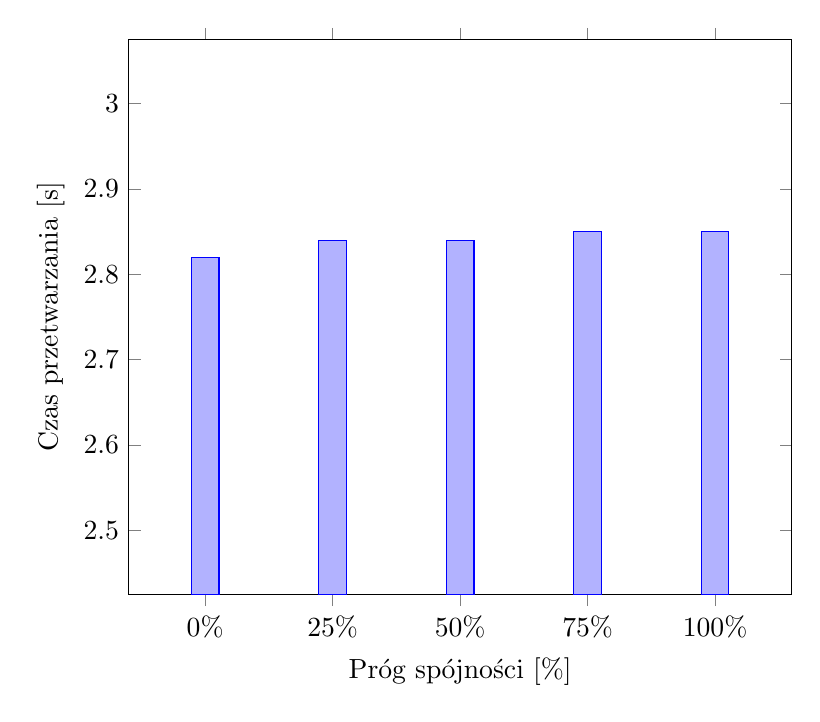
\begin{tikzpicture}
        \begin{axis}[
            width=10cm,
            ymin=2.5, ymax=3,
%             xtick={0, 25, 50, 75, 100},
            xticklabels={0, 0, 0\%, 25\%, 50\%, 75\%, 100\%},
            enlargelimits=0.15,
            ylabel={Czas przetwarzania [s]},
            xlabel={Próg spójności [\%]},
            ybar
        ]
            \addplot plot coordinates {(1,2.82) (2,2.84) (3,2.84) (4,2.85) (5,2.85)};
        \end{axis}
        \end{tikzpicture}
     
    \end{figure}

    \paragraph{}
    Z przeprowadzonych badań można wywnioskować, że w przypadku badanych obrazów najbardziej skuteczne parametry to liczność sąsiedztwa znajdująca się w zakresie (20,50) oraz próg spójności o wartościach około 0,50 (50\%). Nieodpowiedni dobór parametrów może doprowadzić do zbyt rygorystycznej selekcji par punktów spójnych lub do występowania dużej ilości szumu w zbiorze par spójnych. Tak jak wspomniano w badaniach wartość progu spójności nie ma żadnego wpływu na czas przetwarzania, większa liczność sąsiedztwa jednak może znacznie wpłynąć na czas potrzebny do uzyskania wyniku.
    
\end{document}
